\section*{Introduction}

TheSquid is a C library providing structures and functions to perform cluster computing.\\ 

Cluster computing consists of performing the computation of a task by dividing it into several subtasks, ran in parallel on several physical devices and/or independant processes. A process, called the Squad, running on one device request the execution of tasks to one or more processes, called the Squidlets, on the same or other devices. TheSquid is the combination of a Squad and one or more Squidlets. TheSquid library takes care of dividing the main task into subtasks and managing the computation of these subtasks (communication with the Squidlets and processing of the results of subtasks).\\

Available tasks to be computed by TheSquid are:
\begin{itemize}
\item Dummy: a task to perform test
\item Benchmark: a task to benchmark the performance of TheSquid
\item PovRay: a task to render computer graphic image using POV-Ray
\item ResetStats: a task to reset Squidlets' internal statistics
\end{itemize}
The library can be extended to other tasks.\\

TheSquid provides two executable files (\begin{ttfamily}squad\end{ttfamily} and \begin{ttfamily}squidlet\end{ttfamily}). They can be used as stand alone to perform cluster computing, the detail of executed tasks and cluster configuration being given through configuration files in JSON format. The library can also be integrated into another application.\\

TheSquid has been tested on a cluster of Raspberry Pi, however the cluster may be any set of heteregenous devices able to comunicate between each other through TCP/IP protocol. This document describes in detail the implementation on a cluster of Raspberry Pi only.\\

It uses the \begin{ttfamily}PBErr\end{ttfamily}, \begin{ttfamily}PBMath\end{ttfamily}, \begin{ttfamily}GSet\end{ttfamily}, \begin{ttfamily}ResPublish\end{ttfamily}, \begin{ttfamily}PBJson\end{ttfamily}, \begin{ttfamily}PBCExtension\end{ttfamily}, \begin{ttfamily}GenBrush\end{ttfamily} and \begin{ttfamily}PBFileSys\end{ttfamily} libraries.\\

\section{Protocol}

\section{Tasks}

\subsection{File format}

When a task is saved into a text file with JSON format the following properties must be specified:\\
\begin{ttfamily}\{"SquidletTaskType":"1", "id":"1", "maxWait":"1"\}\end{ttfamily}\\
where
\begin{itemize}
\item "SquidletTaskType" is the type of task (see below)
\item "id" is the id of the task
\item "maxWait" is the number of seconds the Sqaud will wait for the result from the Squidlet before giving up and trying again the task on another Squidlet
\end{itemize}
In addition, the data sent by the Squad to the Squidlet as described below must be added.
 
\subsection{Dummy}

Type: 1\\

Data for the task request from the Squad to the Squidlet:\\
\begin{ttfamily}\{"v":"1"\}\end{ttfamily}\\
The value of "v" is actually copied from the "id" and needs not to be specified.\\

Task action: waits for "v" seconds.\\

Data of the result of the task request from the Squidlet to the Squad, if successful:\\
\begin{ttfamily}\{"success":"1","temperature":"0.0","v":"-1"\}\end{ttfamily}\\
where
\begin{itemize}
\item "success" is the success flag
\item "temperature" is the temperature of the device of the Squidlet if available
\item "v" is equal to the opposite of the "v" in the task request
\end{itemize}
If failed:\\
\begin{ttfamily}\{"success":"0","temperature":"0.0","err":"Invalid input"\}\end{ttfamily}\\
where
\begin{itemize}
\item "success" is the failure flag
\item "temperature" is the temperature of the device of the Squidlet if available
\item "err" is the error message
\end{itemize}

\subsection{Benchmark}

Type: 2\\

Data for the task request from the Squad to the Squidlet:\\
\begin{ttfamily}\{"nb":"1", "payloadSize":" "\}\end{ttfamily}\\
where
\begin{itemize}
\item "nb" is the number of sort
\item "payloadSize" is a string whose content is ignored but size is used to set the quantity of data sent over the network
\end{itemize}\\

Task action: sorts "nb" times a set of GSet of 10*length(payloadSize).\\

Data of the result of the task request from the Squidlet to the Squad, if successful:\\
\begin{ttfamily}\{"success":"1","temperature":"0.0","v":"1"\}\end{ttfamily}\\
where
\begin{itemize}
\item "success" is the success flag
\item "temperature" is the temperature of the device of the Squidlet if available
\item "v" is equal to the sorting value of the first element of the sorted GSet
\end{itemize}
If failed:\\
\begin{ttfamily}\{"success":"0","temperature":"0.0","err":"Invalid input"\}\end{ttfamily}\\
where
\begin{itemize}
\item "success" is the failure flag
\item "temperature" is the temperature of the device of the Squidlet if available
\item "err" is the error message
\end{itemize}

\subsection{PovRay}

Type: 3\\

Data for the task request from the Squad to the Squidlet:\\
\begin{ttfamily}\{"SquidletTaskType":"3", "id":"1", "maxWait":"1", \\
"ini":"./testPov.ini", "sizeMinFragment":"100", "sizeMaxFragment":"1000"\}\end{ttfamily}

\subsection{ResetStats}

Type: 4\\

This task is a special task used by the function \begin{ttfamily}SquadRequestSquidletToResetStats\end{ttfamily}.

\subsection{Statistics data in task result}

\section{Setup of the cluster}

This section introduces how to setup and configure a cluster on which to use TheSquid. It is important to remind that TheSquid doesn't necessarily need a physical cluster of devices. One physical device may be used to run all the Squad and Squidlets.\\

\subsection{Raspberry Pi 3B+}

If the OS is not yet installed on the Pi: 
\begin{enumerate}
\item On a PC, download the Raspbian Stretch Lite image (1.9Gb) from \begin{ttfamily}https://www.raspberrypi.org/downloads/raspbian/\end{ttfamily}
\item If not already installed, install Etcher, cf \begin{ttfamily}https://www.balena.io/etcher/\end{ttfamily}
\item Launch Etcher
\item Plug the 8Gb microSD card (should be class 10 or higher for better results)
\item Select the downloaded image
\item Select the microSD card
\item Flash!
\item Create an empy file named \begin{ttfamily}ssh\end{ttfamily} on the boot drive of the miccroSD card
\item Insert the microSD into the Raspberry Pi
\end{enumerate}

Once the OS is intalled on the Pi:
\begin{enumerate}
\item Connect the Raspberry Pi to the network (should use a lan cable of class 7 or more for best results)
\item Turn on the Raspberry Pi
\item Get the IP adress of a PC connected to the local network with ifconfig, lets say its \begin{ttfamily}a.b.c.d\end{ttfamily}
\item Scan the devices on the local network with the command \begin{ttfamily}nmap -sP a.b.c.0/24\end{ttfamily}
\item Connect to the Raspberry Pi through ssh with the command \begin{ttfamily}ssh pi@ip.addr.goes.here\end{ttfamily}, default password is raspberry
\item Setup the Raspberry Pi with \begin{ttfamily}sudo raspi-config\end{ttfamily}
\item Change the password, locale and timezone, expand the file system, and exit
\item Set the hostname with the following commands
\begin{ttfamily}
sudo hostname Squidlet001  # whatever name you chose\\
sudo nano /etc/hostname    # change the hostname here too\\
sudo nano /etc/hosts       # change "raspberrypi" to "Squidlet001"
\end{ttfamily}
\item Ensure the system time is right with the command \begin{ttfamily}sudo apt install ntpdate -y\end{ttfamily}
\item Reboot with the command \begin{ttfamily}sudo reboot\end{ttfamily}
\item Make a directory to clone the git repositories with the command \begin{ttfamily}mkdir ~/GitHub\end{ttfamily}
\item Move to the \begin{ttfamily}~/GitHub\end{ttfamily} directory
\item Clone the repository \begin{ttfamily}PBMake\end{ttfamily} with the command\\
\begin{ttfamily}git clone https://github.com/BayashiPascal/PBMake.git\end{ttfamily}
\item Edit the root Makefile with the command \begin{ttfamily}nano ~/GitHub/PBMake/Makefile.inc\end{ttfamily} and change the value of \begin{ttfamily}ROOT\_DIR\end{ttfamily} with \begin{ttfamily}/home/pi/GitHub/\end{ttfamily} and the value of \begin{ttfamily}BUILD\_ARCH\end{ttfamily} with \begin{ttfamily}2\end{ttfamily}
\item Clone the repository \begin{ttfamily}TheSquid\end{ttfamily} with the command\\
\begin{ttfamily}git clone https://github.com/BayashiPascal/TheSquid.git\end{ttfamily}
\item Move to the \begin{ttfamily}~/GitHub/TheSquid\end{ttfamily} directory
\item Open the Makefile with the command \begin{ttfamily}nano Makefile\end{ttfamily} and make sure the \begin{ttfamily}BUILD\_MODE\end{ttfamily} is set to \begin{ttfamily}1\end{ttfamily}
\item Compile the repository TheSquid with the command \begin{ttfamily}make\end{ttfamily}, others repository are automatically installed
\item Check everything works fine with \begin{ttfamily}./main\end{ttfamily}.
\item Install \begin{ttfamily}lsof\end{ttfamily} with \begin{ttfamily}sudo apt update \&\& sudo apt install lsof\end{ttfamily}
\end{enumerate}

To exchange data between devices during computation, a common file system will be necessary. Below is given the example of how to mount a NAS station:
\begin{enumerate}
\item \begin{ttfamily}sudo mkdir /mnt/NAS\end{ttfamily}
\item \begin{ttfamily}sudo nano /etc/fstab\end{ttfamily}
\begin{ttfamily}//<IP\_TO\_NAS>/TheSquid /mnt/NAS cifs \\
user,uid=1000,rw,suid,credentials=/etc/credentials 0 0\end{ttfamily}
\item \begin{ttfamily}sudo nano /etc/credentials\end{ttfamily}
\begin{ttfamily}username=squidlet\end{ttfamily}
\begin{ttfamily}password=mypassword\end{ttfamily}
\item \begin{ttfamily}sudo apt-get -y install cifs-utils\end{ttfamily}
\end{enumerate}

If you wish to use the PovRay task to render computer graphics using TheSquid, you need to install POV-Ray:
\begin{enumerate}
\item sudo apt-get -y update
\item sudo apt-get -y install libboost-all-dev
\item sudo apt-get -y install zlib1g-dev
\item sudo apt-get -y install libpng-dev
\item sudo apt-get -y install libjpeg8-dev
\item sudo apt-get -y install libopenexr-dev
\item sudo apt-get -y install libtiff5-dev libtiff5 libjbig-dev
\item sudo apt-get -y install autoconf
\item cd ~/GitHub
\item git clone https://github.com/POV-Ray/povray.git
\item cd ~/GitHub/povray/unix/
\item git checkout 3.7-stable
\item ./prebuild.sh
\item cd ../
\item ./configure COMPILED\_BY="TheSquid $<$email@address$>$" --with-boost-libdir=/usr/lib/arm-linux-gnueabihf
\item make
\item sudo make install
\item make check
\end{enumerate}

\section{Performance}

\subsection{PC}

Benchmark executed on two Squidlets running on the same PC has the Squad, compared to the benchmark executed on this PC without using TheSquid.

\begin{center}
\begin{figure}[H]
\centering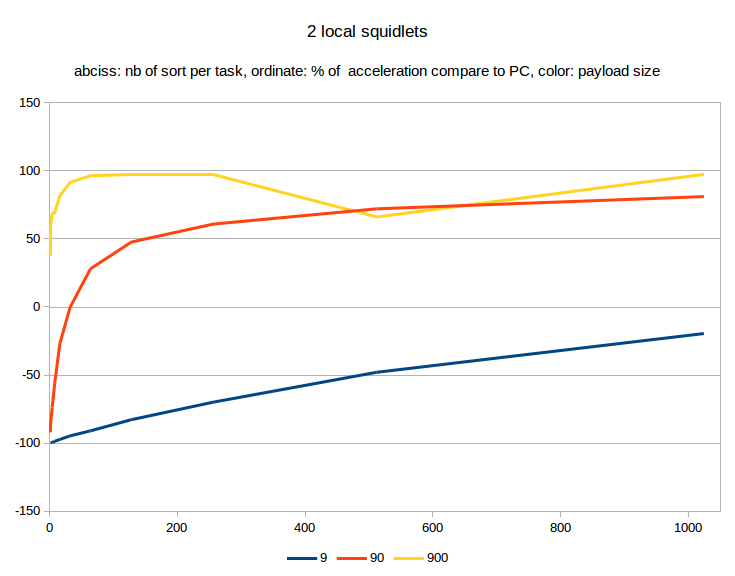
\includegraphics[width=10cm]{./benchmark01.png}\\
\end{figure}
\end{center}

For a payload of 9 bytes, the execution is slower when using TheSquid whatever the number of sorts per task. The time lost during communication between the Squad and the Squidlets, and the time lost managing the subtasks overcome the gain of running subtasks in parallel.\\

For a payload of 90 and 900 bytes, the gain of running subtasks in parallel quickly overcomes the lost and the gain converges toward the expected 100\% (given that the PC had a quadcore processor, i.e. running two Squidlets locally was equivalent to running simultaneously two benchmarks compare to one for the reference without TheSquid).\\

\subsection{Raspberry Pi 3B+}

Benchmark executed on two Squidlets running on the same PC has the Squad plus 24 Squidlets running on 6 Raspbery Pi (4 Squidlets per Pi which are quadcore), compared to the benchmark executed on the PC without using TheSquid.

\begin{center}
\begin{figure}[H]
\centering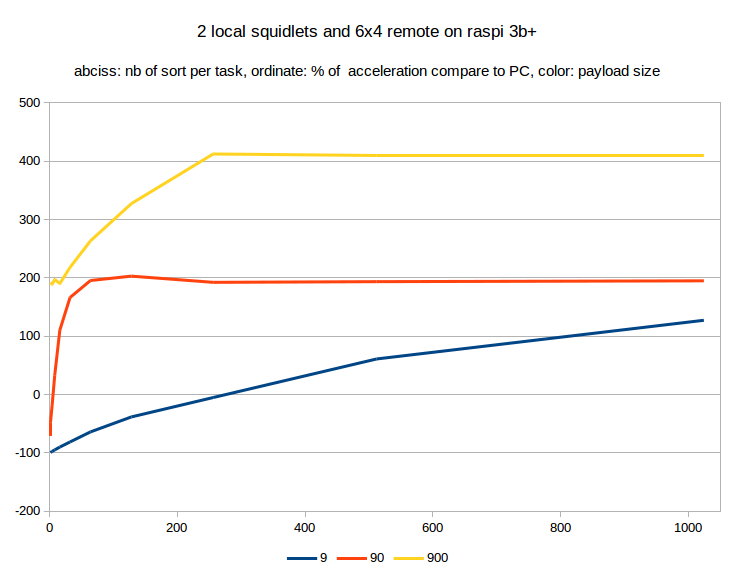
\includegraphics[width=10cm]{./benchmark02.png}\\
\end{figure}
\end{center}

For a payload of 9 bytes, the execution on TheSquid starts to perform faster from around 300 sorts per tasks. The gain converges toward a little more 100\%. For payloads of 90 and 900 bytes, the gain gets positive from, resp., 1 and 10 sorts per tasks, converging toward, resp., 200\% and 400\%.\\

Compare to two squidlets on the same PC, using a cluster of Raspberry Pi shows that the lost of performance due to network communication and task management is non negligeable if the tasks are small, but the gain can be important if the tasks get big enough.\\

The size from which TheSquid is getting advantageous depends on the hardware specification and cannot be foreseen, thus the user is adviced to run the benchmark on its own cluster to appreciate it. The benchmark function could also be used to estimate the gain of new tasks developped in the future.\\ 

\section{Interface}

\begin{scriptsize}
\begin{ttfamily}
\verbatiminput{/home/bayashi/GitHub/TheSquid/thesquid.h}
\end{ttfamily}
\end{scriptsize}

\section{Code}

\subsection{thesquid.c}

\begin{scriptsize}
\begin{ttfamily}
\verbatiminput{/home/bayashi/GitHub/TheSquid/thesquid.c}
\end{ttfamily}
\end{scriptsize}

\subsection{squidlet.c}

\begin{scriptsize}
\begin{ttfamily}
\verbatiminput{/home/bayashi/GitHub/TheSquid/squidlet.c}
\end{ttfamily}
\end{scriptsize}

\subsection{squad.c}

\begin{scriptsize}
\begin{ttfamily}
\verbatiminput{/home/bayashi/GitHub/TheSquid/squad.c}
\end{ttfamily}
\end{scriptsize}

\section{Makefile}

\begin{scriptsize}
\begin{ttfamily}
\verbatiminput{/home/bayashi/GitHub/TheSquid/Makefile}
\end{ttfamily}
\end{scriptsize}

\section{Unit tests}

\begin{scriptsize}
\begin{ttfamily}
\verbatiminput{/home/bayashi/GitHub/TheSquid/main.c}
\end{ttfamily}
\end{scriptsize}

\section{Unit tests output}

\begin{scriptsize}
\begin{ttfamily}
\verbatiminput{/home/bayashi/GitHub/TheSquid/unitTestRef.txt}
\end{ttfamily}
\end{scriptsize}

